\documentclass{beamer}
\graphicspath{{../graphics/}}
\usepackage{listings}
\usepackage{ulem}

\newcommand{\linespace}{\vspace{1em}}

\mode<presentation>
{
  \usetheme{Darmstadt}
  \setbeamertemplate{footline}[frame number]
  \setbeamertemplate{navigation symbols}{}
  \setbeamercovered{transparent}
}

\AtBeginSection[]
{
   \begin{frame}
        \frametitle{Table of Contents}
        \tableofcontents[sectionstyle=show/hide,subsectionstyle=show/show/hide]
   \end{frame}
}

%\usepackage[danish]{babel}
\usepackage[T1]{fontenc}

\usepackage[utf8]{inputenc}

\usepackage{times}

\usepackage{tikz}

\title[Mapping med Lego-robot]{Mapping med Lego-robot}

\subtitle{SW505E13}

\author[SW505E13]{Mikkel Sand\o ~Larsen, \and Bruno Thalmann, \and Stefan Marstrand Getreuer Micheelsen, \and Stefan Thilemann, \and Mikael Elki\ae r Christensen, \and Anders R. Nielsen}

\institute[Aalborg University]
{
  Department of Computer Science\\
  Aalborg University}

\date[CFP 2003]{31. Januar 2014}

\begin{document}

%--------------------------------------------------
%     INTRODUKTION
%--------------------------------------------------

\begin{frame}
  \titlepage
\end{frame}

\begin{frame}
    \frametitle{Table of Contents}
    \tableofcontents[sectionstyle=show/show,subsectionstyle=hide/hide/hide]
\end{frame}

\section{Overblik}

%--------------------------------------------------
%     BAGGRUND
%--------------------------------------------------
\subsection{Baggrund}
\begin{frame}[fragile]{Anvendelse}
	Stort anvendelsesområde for robotter
	\begin{itemize}
		\item Industri
			\begin{itemize}
			\item Droner (overvågning/kortlægning)
			\item Lager robotter
			\end{itemize}
		\item Privat
			\begin{itemize}
			\item Støvsuger robotter
			\item Plæneklipper robotter
		\end{itemize}
	\end{itemize}
\end{frame}

\begin{frame}[fragile]{Grundlæggende problemstillinger}
	\begin{columns}
		\begin{column}{0.5\textwidth}
			Krav til robotten så den kan begå sig i dens omgivelser
			\linespace
			\begin{itemize}
				\item Lokation (interaktion med omgivelser)
				\item En form for kort (til navigation)
			\end{itemize}
		\end{column}
		\pause
		\begin{column}{0.5\textwidth}
			SLAM (\textbf{S}imultaneous \textbf{L}ocalization \textbf{A}nd \textbf{M}apping)
			\linespace
			\begin{itemize}
				\item \textit{Svært!}
					\begin{itemize}
						\item Approximering af lokation
					\end{itemize}
				\item Lokation afhængig af kort, og omvendt
			\end{itemize}
		\end{column}
\end{columns}
\end{frame}


\subsection{Problem}
%--------------------------------------------------
%     AFGRÆNSNING
%--------------------------------------------------
\begin{frame}[fragile]{Afgrænsning}
	\begin{itemize}
		\item Lokalisering vha. color-tracking fra Kinect
	\end{itemize}
	
	\linespace
	\pause
	
	Simplificering af robottens kørselsmiljø:
	\begin{itemize}
		\item Robottens verden er 90 grader
		\item Verdenen er et afgrænset område
		\item Verdenen er plan og befinder sig indendørs
	\end{itemize}
	\linespace
	Mindsker kravene til robotten og gør det nemmere at evaluere resultater.
\end{frame}

%--------------------------------------------------
%     PROBLEMFORMULERING
%--------------------------------------------------
\begin{frame}[fragile]{Problemformulering}
	\begin{center}
		\textit{Hvordan kan der konstrueres software til en robot, hvis formål er at kortlægge en ukendt verden, forudsat at den til enhver tid kender sin position?}
	\end{center}
\end{frame}

%--------------------------------------------------
%     MÅLSÆTNING
%--------------------------------------------------
\begin{frame}[fragile]{Målsætning}
	Grundlag for evaluering af det endelige produkt:
	\begin{itemize}
	\item To forskellige overvejelser
		\begin{itemize}
			\item Hastighed af kortlægning
			\item Præcision af kortlægning
		\end{itemize}
	\end{itemize}
	\linespace
	\pause
	
	Målet med dette projekt:
	\begin{itemize}
		\item At bygge en robot, der kan konstruere et præcist kort
	\end{itemize}
	\linespace
	\pause
	
	Vurdering af valgte målsætning:
	\begin{itemize}
		\item \textit{Det skal være muligt at navigere alene ud fra informationen i kortet og køre fra et hjørne til det diagonalt modsatte}
	\end{itemize}
\end{frame}

%--------------------------------------------------
%     FORSØGSOPSTILLING
%--------------------------------------------------
\subsection{Forsøgsopstilling}
\begin{frame}[fragile]{Kørselsmiljø set fra siden}
	\begin{figure}
		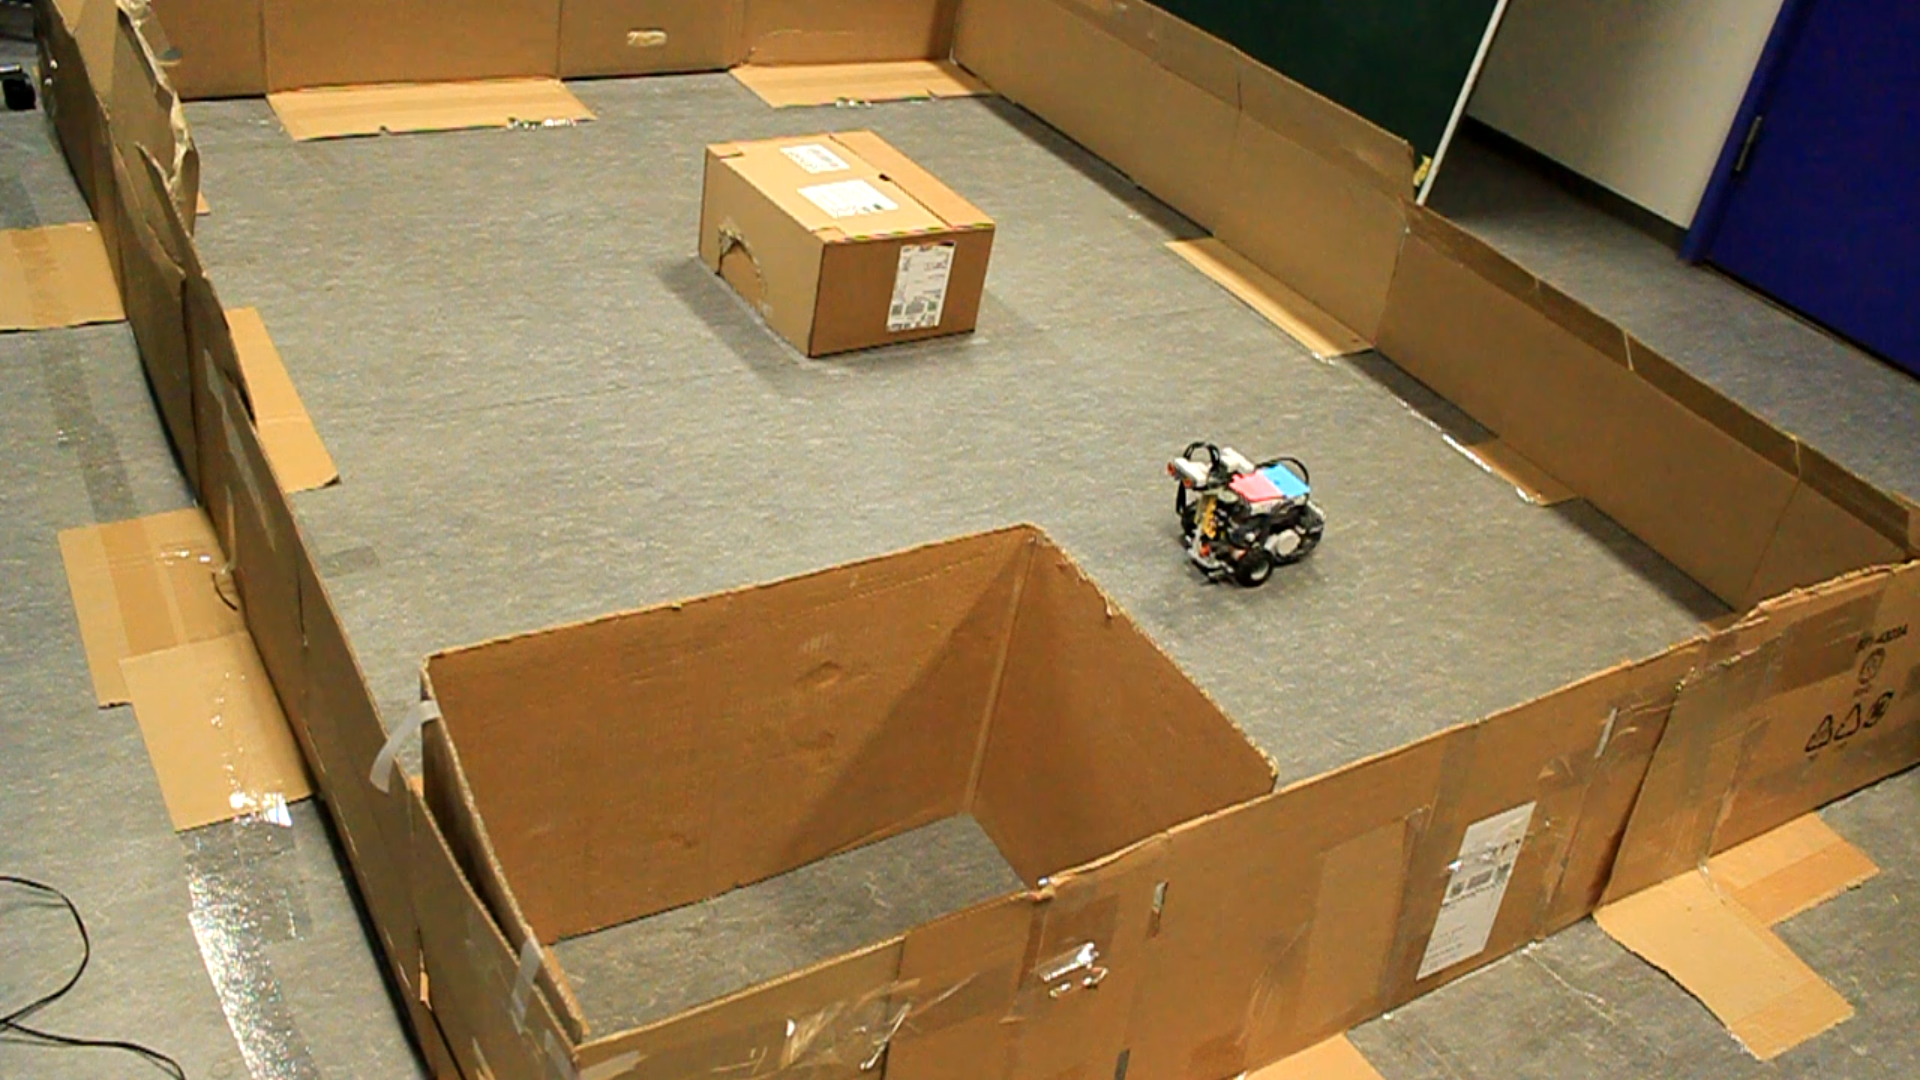
\includegraphics[width=1\textwidth]{verden/opstilling.png}
	\end{figure}
\end{frame}

\begin{frame}[fragile]{Forsøgsopstilling og Kinect}
	\begin{columns}
		\begin{column}{0.5\textwidth}
			\begin{itemize}
				\item Kørselsmiljø set fra Kinect
			\end{itemize}
			\begin{figure}
				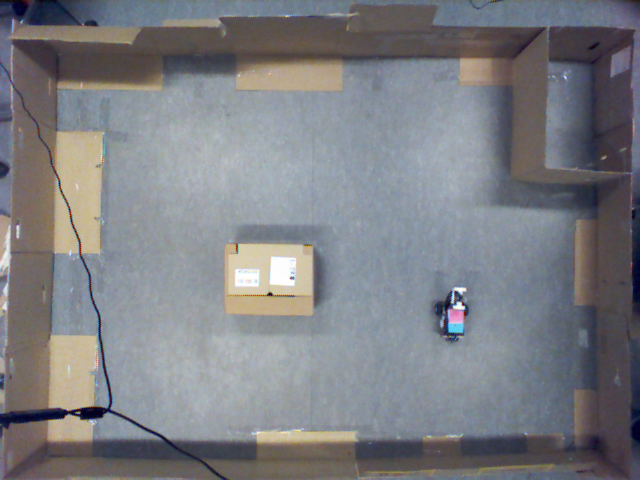
\includegraphics[width=1\textwidth]{evaluering/emptyGrid.png}
			\end{figure}
		\end{column}
		
		\begin{column}{0.5\textwidth}
				\begin{itemize}
					\item Montering af Kinect i loft
				\end{itemize}
			\begin{figure}
				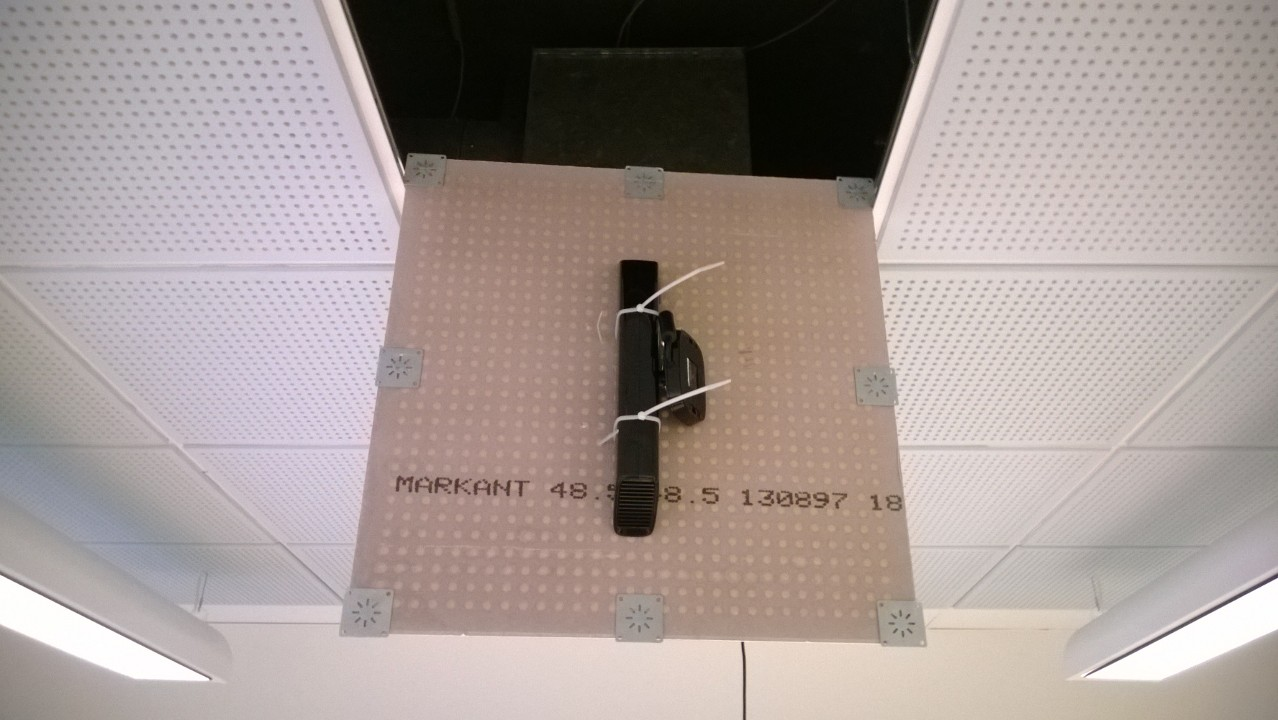
\includegraphics[width=1\textwidth]{verden/kinect.jpg}
			\end{figure}
	\end{column}
\end{columns}
\end{frame}

%--------------------------------------------------
%     EVALUERINGSMETODE
%--------------------------------------------------
\subsection{Evaluering af målsætning}
\begin{frame}[fragile]{Vurderingsmål}
	\begin{itemize}
		\item Approximering af et optimalt kort for forsøgsopstillingen
	\end{itemize}
	
	\begin{figure}
		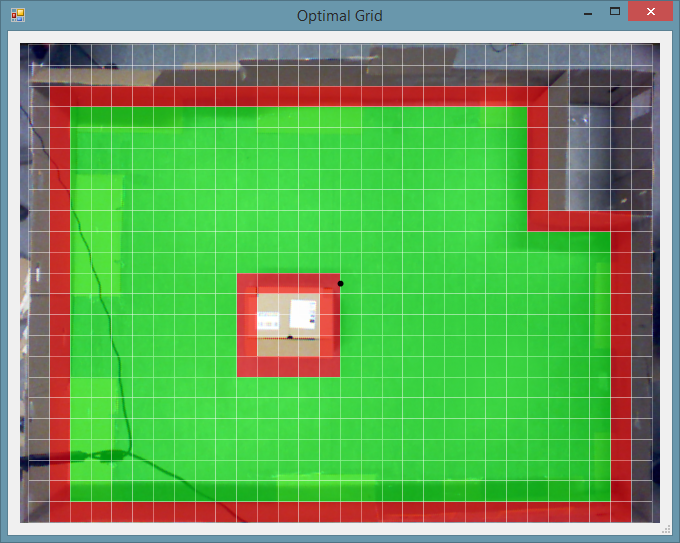
\includegraphics[width=.65\textwidth]{evaluering/optimalgrid.png}
	\end{figure}
\end{frame}
\end{document}